\documentclass[tikz,border=2pt]{standalone}
\usetikzlibrary{decorations.markings}
\usetikzlibrary{positioning}
\usepackage{tkz-euclide}
\usepackage{amsmath}
% \newcommand*\mydrawellipse[3]{%
%     \draw[dotted,thick] (#2) arc[start angle=0,delta angle=180,x radius=#3 cm,y radius=\fpeval{#3 / 4}cm] (#1);
%     \draw[thick] (#1) arc[start angle=180,delta angle=180,x radius=#3 cm,y radius=\fpeval{#3 / 4}cm] (#2);
% }
\newcommand*\mydrawellipse[3][0.15]{%
    \tkzCalcLength(#2,#3)%
    \tkzGetLength{distance}%
    \draw[dotted,thick] (#3) arc [start angle=0,delta angle=180,x radius=\fpeval{\distance/2} cm,y radius=\fpeval{\distance * (#1)}cm] (#2);
    \draw[thick] (#2) arc[start angle=180,delta angle=180,x radius=\fpeval{\distance/2} cm,y radius=\fpeval{\distance * (#1)}cm] (#3);
}

\begin{document}

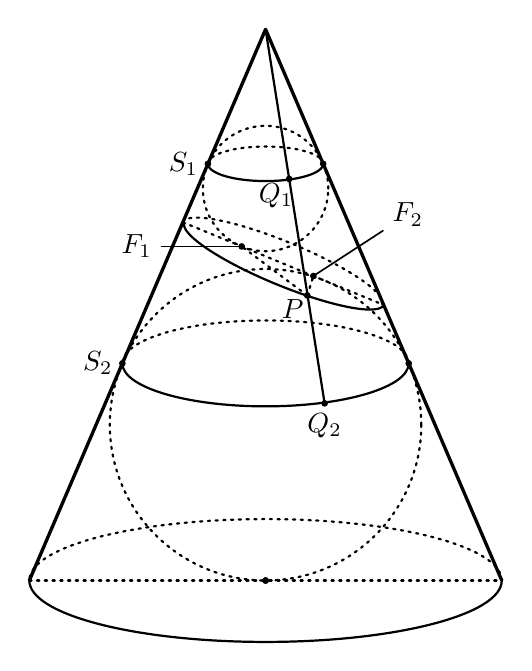
\begin{tikzpicture}[line cap=round,line join=round]
\tkzDefPoint(0,7){H}
\tkzDefPoint(-3,0){A}
\tkzDefPoint(3,0){B}
\tkzDefPoint(0,0){O}
% \tkzDrawPolygon[very thick](H,A,B)
\tkzDrawSegments[very thick](H,A H,B)
\tkzDrawSegments[thick,dotted](A,B)

\tkzDefPointWith[linear,K=0.65](A,H)
\tkzGetPoint{Z1}
\tkzDefPointWith[linear,K=0.65](B,H)
\tkzGetPoint{Z1'}
\tkzDefPointWith[linear,K=0.5](A,H)
\tkzGetPoint{Z2}
\tkzDefPointWith[linear,K=0.5](B,H)
\tkzGetPoint{Z2'}
\tkzDrawSegment[thick,dotted](Z1,Z2')
% \tkzDrawPoints[color=red](A,B,H,Z1,Z1',Z2,Z2')

\tkzDefSpcTriangle[intouch,name=X](A,B,H){_a,_b,_c}
\tkzDefCircle[in](A,B,H)
\tkzGetPoints{O2}{o2}
\tkzDrawCircle[thick,dotted,black](O2,o2)

\tkzDefSpcTriangle[intouch,name=Y](Z1,Z2',H){_a,_b,_c}
\tkzDefCircle[in](Z1,Z2',H)
\tkzGetPoints{O1}{o1}
\tkzDrawCircle[thick,dotted,black](O1,o1)

\mydrawellipse[0.13]{A}{B}
\mydrawellipse{X_b}{X_a}
\mydrawellipse{Y_b}{Y_a}

\tkzDefPointWith[linear,K=0.65](Z1,Z2')
% F1 = Y_c
\tkzGetPoint{F2}

\tkzCalcLength(Z1,Z2') \tkzGetLength{mydistance}%
\tkzFindAngle(Z1,Z2',Z2) \tkzGetAngle{myangle}
\draw[thick,rotate=-\myangle] (Z2') arc[start angle=0,delta angle=-180,x radius=\fpeval{\mydistance/2-.01} cm,y radius=\fpeval{\mydistance * 0.1}cm] (Z1);
\draw[thick,rotate=-\myangle,dotted] (Z1) arc[start angle=180,delta angle=-180,x radius=\fpeval{\mydistance/2-.01} cm,y radius=\fpeval{\mydistance * 0.1}cm] (Z2');

\tkzDefPoint(.75,2.25){Q2}
\tkzDrawSegment[thick](H,Q2)
\tkzDefPoint(.53,3.62){P}
\tkzDrawSegments[thick,dotted](P,Y_c P,F2)
\tkzDefPoint(.3,5.1){Q1}


\node[left] at (Y_b) {$S_1$};
\node[left] at (X_b) {$S_2$};
\tkzLabelPoint[below](Q2){$Q_2$}
\tkzLabelPoint[below left=-3pt](P){$P$}
\tkzLabelPoint[below left=-2pt and -5pt](Q1){$Q_1$}

\node [pin={[pin distance=1cm,pin edge={semithick,black}]left:$F_1$},inner sep=0pt,outer sep=0pt] at (Y_c) {};
\node [pin={[pin distance=1cm,pin edge={semithick,black}]30:$F_2$},inner sep=0pt,outer sep=0pt] at (F2) {};

\tkzDrawPoints[color=black](Y_a,Y_b,Y_c)
\tkzDrawPoints[color=black](X_c,F2)
\tkzDrawPoints[color=black](X_a,X_b,X_c)
\tkzDrawPoints[color=black](Q1,Q2,P)
\end{tikzpicture}

\end{document}